\section{Methodology and theory}
\label{sec:problem_description}

\subsection{实验流程}
\begin{center}
    \begin{tikzpicture}[node distance=1.5cm,
        box/.style={
            rectangle,
            rounded corners,
            draw=black, very thick,
            text width=15em,
            minimum height=2em,
            text centered},
        arrow/.style={
            thick,
            ->,
            >=stealth}
        ]
    
        \node (collect) [box] {采集数据};
        \node (mix) [box, below of=collect] {标记数据};
        \node (train) [box, below of=mix] {训练模型};
        \node (test) [box, below of=train] {测试集测试};
        \node (evaluate) [box, below of=test] {标本评估};
        \node (rate) [box, below of=evaluate] {得出切削良品率};
        \node (improve) [box, below of=rate] {改进与提升};
        
        \draw [arrow] (collect) -- (mix);
        \draw [arrow] (mix) -- (train);
        \draw [arrow] (train) -- (test);
        \draw [arrow] (test) -- (evaluate);
        \draw [arrow] (evaluate) -- (rate);
        \draw [arrow] (rate) -- (improve);
        
        \end{tikzpicture}
    \end{center}
    
\textbf{采集数据:}使用切片机对已预先从生物实验室制备好经过染色处理后石蜡包埋好的组织切片,按照切片机的操作手册进行切片操作,得到切片并记录切削参数。然后转移切片到显微镜下,拍摄切片图像。

\textbf{标记数据:}对采集到的图像数据根据质量的好坏和能否用于生物学观察和分析进行标记。

\textbf{训练模型:}尝试不同结构和形式的深度学习卷积模型,对标记好的数据进行训练。然后监测训练过程中的准确率和损失函数,评估模型性能。

\textbf{测试集测试:}使用测试集对训练好的模型进行测试,评估模型的泛化能力。

\textbf{标本评估:}对另外准备的测试集进行评估,观察模型的实际应用效果,计算模型预测准确率。

\textbf{得出切削良品率:}使用预先准备好的不同角度下的切片图像数据,使用模型进行评估,得出不同角度下的切削良品率,确定最佳切削角度。

\textbf{改进与提升:}根据评估结果,对模型进行调整和改进,提高模型的准确率和泛化能力。

\subsection{图像处理方法}

对于获取的图像数据,可以应用适当的图像预处理。在保持图像完整性和质量的前提下,可以实施某些处理以突出计算机识别的特征,并在一定程度上去除无关特征和噪声。这增强了后续深度学习模型的准确性。

图像分割是图像处理中的关键步骤,目的是将图像划分为几个有意义的区域以进行进一步的分析和处理。在关注生物组织产率的模型中,需要将生物切片分割为生物组织和石蜡区域,强调生物组织部分。

常见的图像分割算法包括边缘检测和阈值分割。

\subsubsection{边缘检测}
对于生物组织切片,质量的关键指标是切片边缘的清晰度。切片边缘的完整性和连续性可以反映样本是否存在质量问题。

有许多边缘检测的算法,如Sobel、Laplacian和Canny算子 \cite{3.1}。

\textbf{Sobel算子}是一种一阶差分算子,可以用来检测图像边缘 \cite{补充1}。假设有一个一维图像$f(x)$,其强度与像素坐标$x$的关系可以如图1所示。在\autoref{fig:original_function}中可以观察到,斜率在x=2.2附近最大,表明在这个点附近图像强度有突然的变化(存在边缘)。取其导数得到一阶导数$f'(x)$,如\autoref{fig:first_derivative}所示,其中导数的绝对值最大。Sobel算子利用这个特性来检测边缘。

\begin{figure}[htbp]
    \centering
    \begin{minipage}[b]{0.32\textwidth}
        \centering
        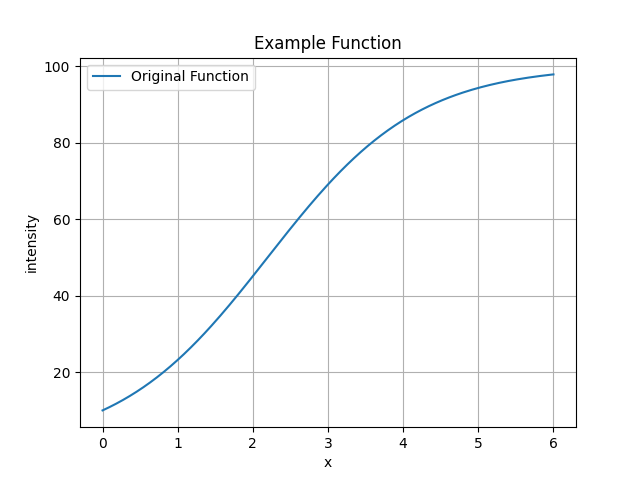
\includegraphics[width=\textwidth]{./fig/original_function.png}
        \caption{f(x)}
        \label{fig:original_function}
    \end{minipage}
    \begin{minipage}[b]{0.32\textwidth}
        \centering
        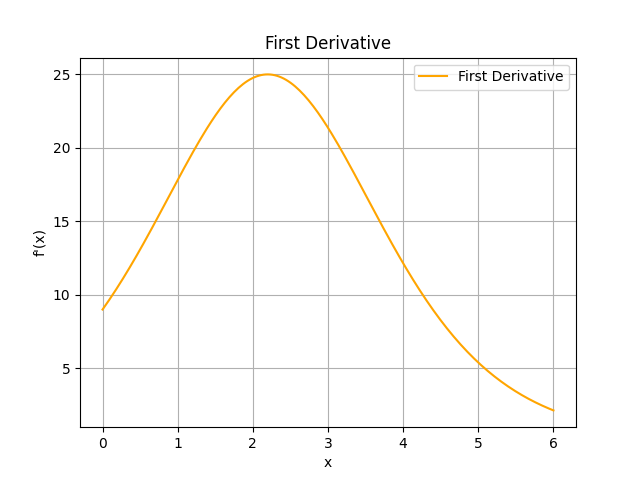
\includegraphics[width=\textwidth]{./fig/first_derivative.png}
        \caption{f'(x)}
        \label{fig:first_derivative}
    \end{minipage}
    \begin{minipage}[b]{0.32\textwidth}
        \centering
        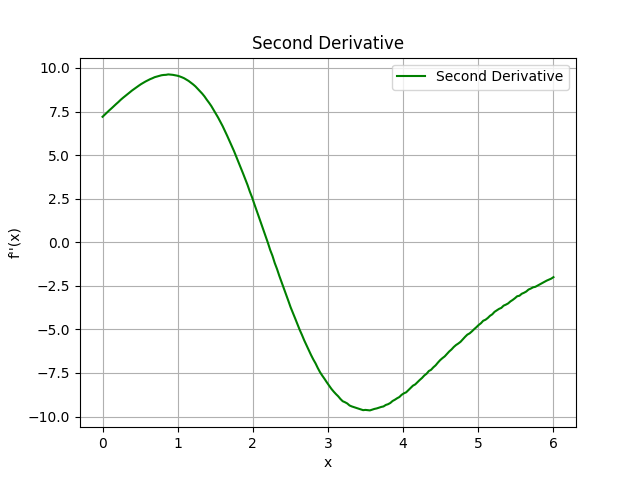
\includegraphics[width=\textwidth]{./fig/second_derivative.png}
        \caption{f''(x)}
        \label{fig:second_derivative}
    \end{minipage}
\end{figure}

\textbf{Laplacian算子}是一种二阶微分算子,其对图像的边缘检测效果较好。它是对sobel算子再进行一次求导得出。在2D图像中,Laplacian算子的定义如下:
\begin{equation}
    \nabla^2 f = \frac{\partial^2 f}{\partial x^2} + \frac{\partial^2 f}{\partial y^2}
\end{equation}
如上图所示,对一阶导数再次求导得到二阶导数$f''(x)$,如\autoref{fig:second_derivative}所示,可以看到在x=2.2左右,二阶导数为0,即说明当laplacian算子$\nabla^2 f$的值为0时,说明图像强度存在突变,即存在边缘。

\textbf{Canny算子}是一种多阶微分算子,他在sobel算子计算后的基础上加入了对噪声的抑制。他由John F. Canny于1986年提出\cite{3.2}.简而言之,其在sobel算子计算后,通过非极大值抑制,滞后阈值等步骤,设置了阈值,排除图像中的假边缘,得到了更加准确的边缘检测结果。

在Experimental work/analytical investigation/ design这一章节中 将会对采集到的图像数据进行三种边缘检测算法的实验,对比其效果。

\subsubsection{阈值分割}

除了边缘检测,还有一种方法是阈值分割。阈值分割是将图像中的像素点分为两类,一类是大于阈值的像素点,另一类是小于阈值的像素点。这种方法适用于图像中的目标和背景的灰度差异较大的情况。

对于样品来说,一个很简单的方法就是将石蜡区域和生物组织区域(样品在制备是已染色)的颜色进行对比,然后通过阈值分割的方法将其分割开来。假定生物组织为黄色,石蜡为白色,那么可以通过设置一个阈值,将图像中的白色部分分割出来,那么剩下的就是生物组织部分。

此外,关于阈值分割还有更多的方法,比如下面就是一个基于Otsu方法的指纹提取算法。将其用在此处能够显著提高生物组织的分割效果。
Yue Yaru和Zhu Jialin 在 《Algorithm of fingerprint extraction and implementation based on OpenCV》一文中提出了一种基于OpenCV的指纹提取算法。该算法对Otsu方法进行了改进,特别是在光照不均匀、图像模糊的情况下能够实现准确、简单、运行时间短的指纹提取。\cite{3.3}

相关的对比和实验将在 Experimental work/analytical investigation/ design这一章节中进行。


\subsection{迁移学习方法的模型选择}

在迁移学习中,常用的预训练模型包括 VGG16, VGG19、Inception等。这些模型已经在像ImageNet这样的大型数据集上进行了大量训练,其中模型中各层的权重已经被优化,可以有效地用于迁移学习。\cite{4.30 7}

\autoref{tab:model_comparison}显示了由牛津大学视觉几何组设计的VGG系列(VGG16,VGG19)模型\cite{DL.5},以及由Google开发的模块化深度学习模型InceptionV3 \cite{DL.6}\cite{DL.7}的参数数量。这些模型拥有大量的参数,使它们能够从复杂的图像中准确地提取特征。利用这些训练有素的模型的能力使研究人员和实践者能够在特定任务上获得高性能,而无需从头开始训练整个网络,既节省了时间和资源,又保持了高准确性。\cite{4.30 8}

\begin{table}[H]
    \centering
    \caption{Comparison of CNN Models}
    \label{tab:model_comparison}
    \begin{tabular}{cccc}
        \toprule
        \textbf{Model} & \textbf{VGG16} & \textbf{VGG19} & \textbf{InceptionV3}\\
        \midrule
        \textbf{Number of Parameters} & 138,357,544 & 143,667,240 & 23,851,784 \\
        \bottomrule
    \end{tabular}
\end{table}

考虑到这些模型都是基于Imagenet数据集训练的,而生物组织切片数据集的特征与Imagenet数据集有很大的不同。对于如何确定最佳模型,则需要通过实验来验证。在Experimental work/analytical investigation/ design这一章节中,将会对这些模型进行实验和性能评估,对比其效果。






